\chapter{Data Processing}
\label{chap:data}

This chapter describes the two datasets, how they were collected and cleaned, what the exploratory analysis revealed, and how additional LLM-assisted labels were created. Several findings here, in particular the sampling biases, determine which features the models may use.

\section{Dataset Description}

\subsection{Steam Reviews Dataset}

The main dataset was collected by the team through the public Steam review API between 21 and 28 September 2026. The target was the 50 most recent positive and 50 most recent negative reviews per game. The final file contains 10,000 reviews of 99 games written between December 2025 and September 2026: 95 games have exactly 100 reviews, while four deviate (Counter-Strike~2: 274, Dota~2: 126, Find The Needle Demo: 66, FiveM: 34), which is why the total is 10,000 rather than $99 \times 100$. Table~\ref{tab:columns} lists the fields; all reviews were identified as English by an automatic language detector.

\begin{table}[!htbp]
\centering
\caption{Fields of the Steam reviews dataset}
\label{tab:columns}
\begin{tabularx}{\textwidth}{lY}
\toprule
\textbf{Field} & \textbf{Description} \\
\midrule
\texttt{app\_id}, \texttt{game\_name} & Steam identifier and name of the game \\
\texttt{review\_id}, \texttt{review\_text} & Review identifier and raw review body \\
\texttt{voted\_up} & Recommendation verdict, used as a proxy label for review sentiment \\
\texttt{playtime\_forever\_hours} & Reviewer's total playtime at crawl time \\
\texttt{votes\_helpful} & Number of ``helpful'' votes received \\
\texttt{timestamp\_created} & Time the review was written \\
\bottomrule
\end{tabularx}
\end{table}

This collection procedure has two consequences that matter throughout the report:
\begin{itemize}
    \item The Recommended/Not Recommended ratio is balanced \textbf{by design} (about 50/50 for most games) and does not reflect each game's real reception, so per-game statistics can only be compared relatively.
    \item Negative reviews are rarer on Steam, so collecting 50 of them required going further back in time. The timestamp and the helpful votes (which accumulate over time) are therefore correlated with the label \textbf{because of the sampling}, not the content. Both are excluded from sentiment models; review age is used only as a control variable for helpfulness.
\end{itemize}

\subsection{Data Stream v2 (Recommendation Data)}

For the recommendation task suggested by the instructor, the data collection members of the team prepared a second file with 299 rows for 100 game entries, normally three reviewers per game from three tiers (users owning the most games, a mid-range user, users owning the fewest games); one entry (7 Days to Die) has no reviewer from the lowest tier, hence 299 rather than 300 rows. Each row contains games owned, reviews written, playtime, helpful and funny votes, the game's overall rating and a review excerpt in Vietnamese. The file shows signs of being simulated (regular text, exactly three reviewers per game, rounded numbers, eight games duplicated with identical rows), Steam IDs lost precision, and every user has a single review. The report therefore treats it as \textbf{illustrative data} for demonstrating recommendation, not as real reviews.

\section{Data Preprocessing and Cleaning}

\subsection{Cleaning the Steam Reviews}

The cleaning removes noise without discarding signals that carry sentiment (Table~\ref{tab:cleaning}). Emoji and censored words are kept because they carry sentiment: the \texttt{<censored>} token appears mostly in negative reviews. A rule flagging long runs of one repeated character was tried and dropped because it mostly caught legitimate texts such as ``-----'', ``!!!!'' or ``yesss''.

\begin{table}[!htbp]
\centering
\caption{Cleaning steps for the Steam reviews dataset}
\label{tab:cleaning}
\begin{tabularx}{\textwidth}{lY>{\RaggedRight\arraybackslash}p{3.4cm}}
\toprule
\textbf{Step} & \textbf{Method} & \textbf{Effect} \\
\midrule
De-duplication & Match texts after lower-casing and collapsing whitespace; keep the first copy; drop duplicate groups with conflicting labels & 29 removed (25 duplicates, 4 conflicts) \\
Markup removal & Remove Steam BBCode tags (keep their content) and URLs; de-duplicate again & 82 reviews modified \\
Normalisation & Replace the heart symbols of Steam's profanity filter by a \texttt{<censored>} token; keep emoji as separate tokens & No empty reviews \\
Quality flags & Truncated, repeated-word spam, too short, mixed language (flagged, not removed) & 20 reviews flagged \\
Name fixes & Normalise misspelled game names & 13 names \\
\bottomrule
\end{tabularx}
\end{table}

The final dataset has \textbf{9,971 reviews} (5,000 Recommended, 4,971 Not Recommended). The median review has 20 words and the mean 54.9 words, a strongly right-skewed distribution.

\subsection{Cleaning Data Stream v2}

Removing the duplicated games leaves \textbf{275 reviews of 92 games}. Reviewers received anonymous identifiers because the original Steam IDs were unusable, and the verdict was recovered from the wording of the rating field and checked against the text. Publishers were joined from an earlier team file (79 of 92 games) and completed manually; genres were assigned manually into 15 groups. The result has 69 publishers, 14 of them with at least two games. Survival (16 games) and builder/management (11) are the largest genres. In this illustrative data, 33\% of the reviews from users owning the fewest games are negative, against 6.5\% for the mid-range tier and none for the tier owning the most games.

\section{Exploratory Data Analysis and Feature Extraction}
\label{sec:eda}

The exploration looked for signals besides the text that relate to sentiment, and for artefacts of the data collection.
\begin{itemize}
    \item \textbf{The text is the main signal.} The strongest non-text feature has a mutual information with the label of only 0.044 (maximum 0.693). The class vocabularies differ clearly: \textit{fun, best, love} versus \textit{censored, boring, worst, crashes}.
    \item \textbf{Longer reviews lean negative} (Spearman $\rho = -0.26$), with the same sign in 96 of the 97 games that have at least 90 reviews.
    \item \textbf{Playtime has an inverted-U relation with sentiment} (Figure~\ref{fig:eda}): reviewers with less than two hours are positive in only 14\% of cases, against 57\% for 10--50 hours. Very short playtime often means refunds or games that do not start.
    \item \textbf{Explicit ``x/10'' scores} are strong but appear in only 4.4\% of reviews; question marks and censored words go with negative reviews.
    \item \textbf{Timestamp and helpful votes} correlate most with the label, but only because of the sampling.
\end{itemize}

\begin{figure}[!htbp]
    \centering
    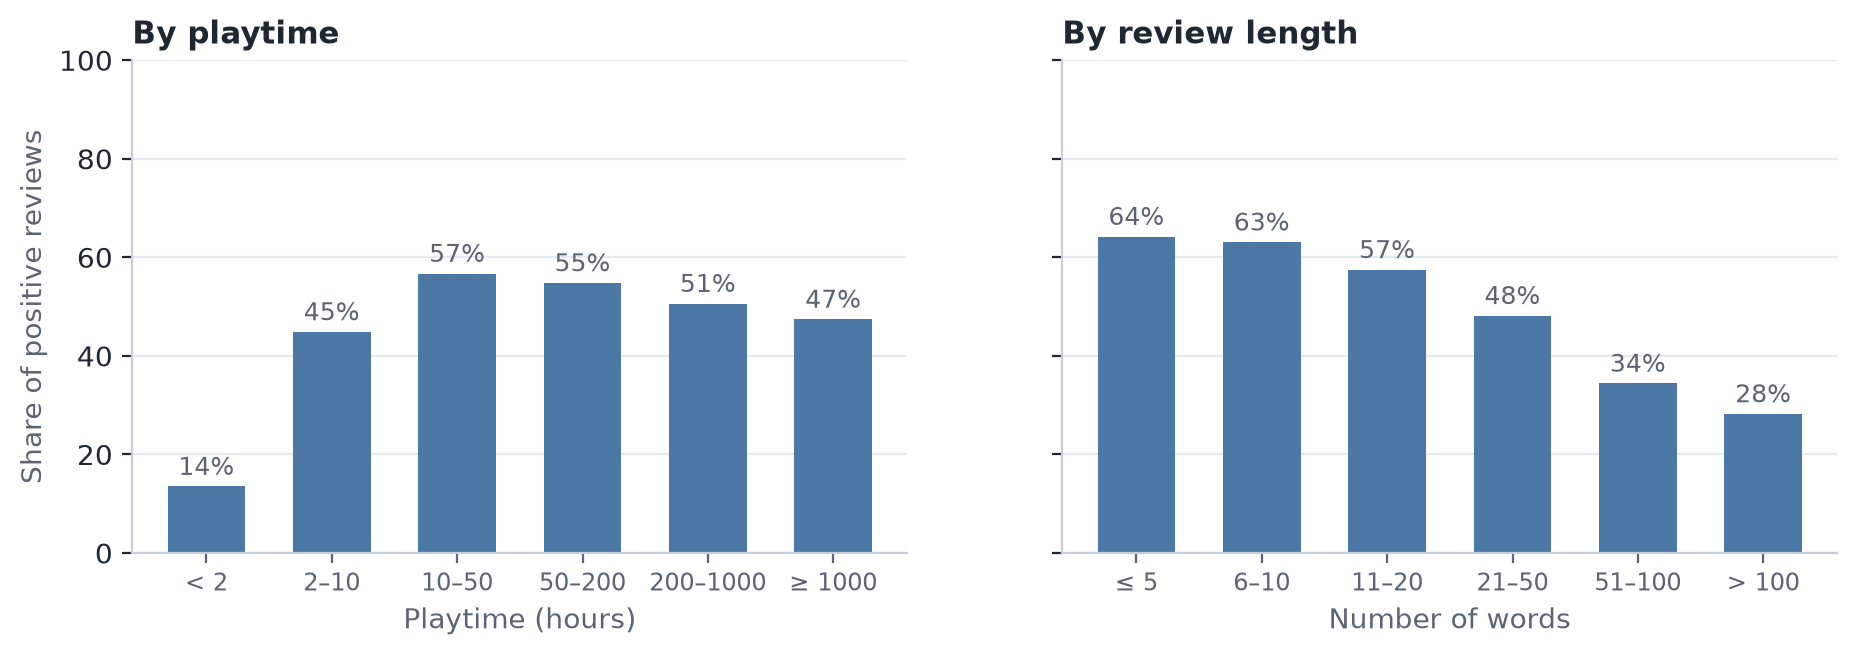
\includegraphics[width=0.9\textwidth]{fig02_eda.png}
    \caption{Share of positive reviews by playtime and by review length.}
    \label{fig:eda}
\end{figure}

From this analysis, ten \textbf{meta features} complement the text: the log word count, presence and value of an x/10 score, presence of a question mark, presence of a censored word, and playtime one-hot encoded into five bins ($<$2h, 2--10h, 10--50h, 50--200h, $\geq$200h). Playtime is binned because of its non-monotonic effect. Text features are learned by the models themselves.

\section{LLM-assisted Annotation}

The Steam verdict describes the whole review, so it cannot train or evaluate aspect-level models, nor tell whether an error comes from the model or from a misleading label. Additional labels were therefore drafted by a large language model (Claude) following written guidelines, without access to the Steam label, the game name or model predictions. The team then \textbf{reviewed every drafted label} (all 500 reviews and all 4,610 sentences) against the guidelines and corrected disagreements. No independent second annotation was made.

\textbf{Review labels.} 500 random reviews from test set A were labelled with a sentiment (217 negative, 187 positive, 71 unclear, 25 mixed) and a type (393 normal, 76 jokes or memes, 15 too short, 8 sarcastic, 8 off-topic). For reviews with a clear sentiment, the label agrees with the Steam verdict in 94.8\% of cases.

\textbf{Sentence labels.} Sentences were labelled with (aspect, polarity) pairs over eight aspects: graphics, audio, gameplay, story, performance/bugs, price/monetisation, online/community and developer; polarity is positive, negative, neutral or unclear. Generic sentences such as ``great game'' get no aspect. Table~\ref{tab:labelsets} lists the sets. Of the 4,610 labelled sentences, 4,461 are used: 97 keyword-selected sentences of an earlier dev split were dropped to keep dev random, and 52 training sentences from reviews that contribute dev sentences were dropped to avoid leakage. These sentence-level labels are independent of the Steam verdict. The keyword lists used as a baseline were written after reading Test 1, which favours them on that set, so Test 2 was labelled only after the keywords were frozen and is the main test set for aspect-level comparisons.

\begin{table}[!htbp]
\centering
\caption{LLM-assisted, team-reviewed labelled data}
\label{tab:labelsets}
\small
\begin{tabularx}{\textwidth}{lrYl}
\toprule
\textbf{Set} & \textbf{Size} & \textbf{Source} & \textbf{Purpose} \\
\midrule
Reviews & 500 & Random, test set A & Error analysis \\
Sentences, Test 1 & 500 & Random, test set A & Evaluation \\
Sentences, extra & 110 & Test set A, keyword-selected & Polarity examples \\
Sentences, Test 2 & 500 & Random, test set A, after keywords were frozen & Main evaluation \\
Sentences, dev & 438 & Random, outside test sets & Model selection \\
Sentences, train & 2,913 & Random, keyword-selected, conflicting & Training \\
\midrule
Sentences, total & 4,461 & 4,610 labelled, 149 unused & \\
\bottomrule
\end{tabularx}
\end{table}

\section{Data Splitting Strategy}
\label{sec:splits}

Two scenarios are used for review-level tasks (Table~\ref{tab:splits}). \textbf{Scenario A (known games)} is a stratified random 70/15/15 split. \textbf{Scenario B (unseen games)} holds out 20\% of the \textit{games} as the test set, which checks whether a model learns general ways of praising and complaining rather than game-specific words such as character or map names.

\begin{table}[!htbp]
\centering
\caption{Data splits for review-level tasks}
\label{tab:splits}
\begin{tabular}{llrrr}
\toprule
\textbf{Scenario} & \textbf{Set} & \textbf{Reviews} & \textbf{\% positive} & \textbf{Games} \\
\midrule
\multirow{3}{*}{A (known games)} & Train & 6,979 & 50.2 & 99 \\
 & Validation & 1,496 & 50.1 & 99 \\
 & Test & 1,496 & 50.1 & 99 \\
\midrule
\multirow{3}{*}{B (unseen games)} & Train & 6,813 & 50.0 & 79 \\
 & Validation & 1,203 & 50.0 & 79 \\
 & Test & 1,955 & 50.7 & 20 \\
\bottomrule
\end{tabular}
\end{table}

All splits use a fixed seed, so every model sees exactly the same data, and vocabularies, TF-IDF weights and scalers are fitted on the training set only. Sentence sets are split by review, and the code checks that no review contributes sentences to both training and dev or test data.
